\chapter{Background and Theory}
% This chapter should describe the theoretical background needed to understand
% and solve the problem. For instance, a description of the hardware platform
% or specific components involved in this assignment, definition of concepts
% that are important to understand the solution should be summarized here. Add
% citations to show sources whenever appropriate, LaTeX and bibliography
% managers make this easy.

This chapter is an introduction to theory and concepts needed to understand the rest of the report. It begins with a section explaining operating systems terminology and a section introducing the Linux operating systems and important system calls. Then it continues with a section on driver programming in Linux. The next section introduces some relevant hardware of the EFM32GG-DK3750 prototyping board, and the final section provides an overview of the PTXdist build system.

\todo{Verify that this is consistent with the rest of the chapter}

\section{Basic Terminology}\label{basic-terminology}
This section introduces some general terminology and concepts concerning operating systems and device drivers in general.

\subsection{Operating Systems}
An operating system is a special piece of software that provides two important functions in a computer:
\begin{itemize}
  \item Managing the hardware resources.
  \item Providing a useful hardware abstraction layer for application programmers.
\end{itemize}
The core of the operating system is called the \emph{kernel} and runs in a privileged software that gives the kernel complete access to all hardware resources. The code running outside the kernel is often referred to as the \emph{user space} or the \emph{userland}, and has only restricted access to hardware. Because of this organization, all hardware-related activities necessary to run the operating system and execute programs is performed by the kernel, and the user space programs only access hardware through the kernel by special \emph{system calls}.
\cite{modern-operating-systems}

\subsection{Device Drivers}
The kernel uses \emph{device drivers} to more easily manage hardware devices with different characteristics. A device driver is a program that manages low-level access to a particular hardware device, providing a clean interface for the rest of the kernel.

\subsection{Kernel Modules}\label{sec:kernel-modules}
The functionality of the kernel may sometimes need to be modified, for instance to accommodate new hardware. While this could be achieved by modifying and rebuilding the kernel, it is often a more attractive alternative to extend the functionality with \emph{kernel modules}, small kernel programs that are loaded at runtime. It is common to write device drivers as kernel modules.

\subsection{Related Terminology}
In addition to the concepts described above, several other terms are used in the context of operating systems:
\begin{description}
\item[Boot Loader] \hfill \\
The bootloader is a small program that runs before the operating system starts, and makes the necessary preparations to load the kernel.
\item[Linux Root Filesystem] \hfill \\
 In Linux, the root filesystem is the filesystem available at the top-level directory. It is denoted with a forward slash, \texttt{/}.
\end{description}

\todo{Things to consider writing about here: \\
\indent - The virtual address space of processes}


\section{Linux}
This section is a brief introduction to important low-level concepts of the Linux operating system, such as system calls and certain Linux devices.

\subsection{The Frame Buffer}\label{sec:the-framebuffer}
The frame buffer device is an abstraction that allows user applications to access the frame buffer of some underlying graphics hardware, and usually appears as \texttt{/dev/fb0}. The pixels displayed on the screen are stored in the frame buffer in a hardware-dependent format, and can be changed by writing to the frame buffer. Frame buffers are \emph{memory devices} and can be mapped into process virtual memory with \texttt{mmap()} as explained in section \ref{mapping-files-to-memory}.

\todo{Add reference to Documentation/fb/framebuffer.txt}


\subsection{Linux System Calls}
This section explains a few Linux system calls relevant in this report.

\subsubsection{Reading and writing files}\label{sec:reading-and-writing-files}
Several system calls in Linux are related to file operations that perform file I/O. This section will introduce some of the most commonly used. The following system calls are available from the headers \texttt{<fcntl.h>} and \texttt{<unistd.h>}.

\begin{description}
\item[\texttt{int open(const char *pathname, int flags);}] \hfill \\
Before any file operations can be performed on a file, a call to \texttt{open()} is needed to allocate the necessary system resources. Here \texttt{pathname} is the absolute path to the file, and \texttt{flags} specify access modes such as read-only or read-write. On success, \texttt{open()} will return a file descriptor that is used as a handle on the file in future system calls.
\item[\texttt{ssize\_t read(int fd, void *buf, size\_t count);}] \hfill \\
After opening a file, the contents of the file can be read as individual bytes with \texttt{read()}. Here \texttt{fd} is the file descriptor previously returned from \texttt{open()}, \texttt{buf} is a buffer where the file contents should be stored, and \texttt{count} is the number of bytes to read from the file. The returned value is the number of bytes that was read into \texttt{buf}. Note that \texttt{read()} gives no guarantee that the requested number of bytes has actually been read into \texttt{buf}. It is up to the application programmer to provide such guarantees by checking the return value.
\item[\texttt{ssize\_t write(int fd, const void *buf, size\_t count);}] \hfill \\
To write bytes to a file, the very similar function \texttt{write()} can be used. The parameters roles are slightly changed: \texttt{buf} is a buffer containing the contents to write to the file, \texttt{count} specifies the number of bytes to write, and the value returned is the actual number of bytes written. As expected, \texttt{fd} is the file descriptor.
\item[\texttt{off\_t lseek(int fd, off\_t offset, int whence);}] \hfill \\
Read and write operations on a file is performed at the bytes located at a specific offset from the beginning of the file, called the \emph{file offset}. The file offset is initially zero, and is incremented with the number of bytes read or written by a file operation. To operate on bytes in a noncontiguous fashion, the offset can be changed with a call to \texttt{lseek()}. Here the meaning of \texttt{offset} depends on the parameter \texttt{whence}. Three possible options are to specify the new offset directly, relative to the current offset, or relative to the end of the file.
\item[\texttt{int close(int fd);}] \hfill \\
After an application is done with a file it should call \texttt{close()} to release the file's associated resources. This will invalidate the file descriptor.
\end{description}

\subsubsection{Mapping files to memory}\label{mapping-files-to-memory}
Accessing a file in an arbitrary manner using the system calls described in section \ref{sec:reading-and-writing-files} will involve many redundant calls to \texttt{lseek()}. A better alternative then is to map the file into the virtual address space of the process, allowing the file to be accessed with ordinary memory accesses. The following system calls are available from the headers \texttt{<sys/mman.h>} and \texttt{<unistd.h>}.

\begin{description}
\item[\texttt{void *mmap(void *addr, size\_t length, int prot, int flags, int fd, off\_t offset);}]
The function \texttt{mmap()} can be used to map a number of \texttt{length} bytes from the file specified by the file descriptor \texttt{fd} into memory. The mapping starts \texttt{offset} bytes from the beginning of the file. Optionally, \texttt{addr} can be used to give the kernel a hint as to where the mapping should be placed in virtual memory, or it can be \texttt{NULL}. \texttt{prot} is a bit field specifying the memory protection of the mapping, and \texttt{flags} sets the visibility of updates to the mapping to other processes.
\item[\texttt{int msync(void *addr, size\_t length, int flags);}] \hfill \\
Updates to a memory mapped file might not become visible immediately. To synchronize a file with a memory map, the application should call \texttt{msync()}.
\item[\texttt{int munmap(void *addr, size\_t length);}] \hfill \\
After the application is done with the memory map, it may call \texttt{unmap()} to delete the mapping and release its associated resources. This will also synchronize the file with the memory map.
\end{description}


\subsection{Asynchronous Signalling}\label{sec:asynchronous-signalling}

\subsubsection{Signals}
\todo{Write about signals in Unix/Linux}



\section{Writing Device Drivers for Linux}\label{writing-device-drivers-for-linux}
This section is a brief introduction to device driver development for the Linux kernel. It begins by explaining some practical details regarding driver development, then it highlights some important parts of the Linux kernel and common programming constructs, and finally it provides a brief outline on driver design. The main focus is on drivers implemented as kernel modules. For an explanation on the terminology used in this section, see section \ref{basic-terminology}.

\todo{Verify that this is consistent with the rest of the chapter}


\subsection{Programming in the Kernel}
Kernel modules are different from user space applications in several important ways, and there are some considerations to take into account when writing a module.

\subsubsection{Module bugs are more serious}
As a module is a part of the kernel, it runs in privileged mode with access to all hardware. A natural consequence of this is that bugs are much more serious. A module bug can easily crash the whole system, for instance by overwriting other parts of the kernel code in memory. Or, perhaps worse, a bug might introduce a security hole.

\subsubsection{Modules cannot link user space code}
Again, because a module runs in privileged mode, it cannot be linked against any user space code. This includes the standard C library with all its nice functions such as \texttt{malloc()}, \texttt{strcmp()} and \texttt{printf()}. Instead, the module is linked against the kernel and has access to kernel routines.

\subsubsection{Module debugging is different}
Debugging a module is different from using ordinary software debuggers such as the GNU Debugger. The Linux kernel must be debugged with the built-in kernel debugger.

\subsubsection{Modules must are linked against the kernel source tree}
Since modules are linked against the kernel, the developer must have a kernel source tree available to build it against. The process of manually downloading, configuring and building a kernel source tree involves a fair amount of work, especially for a novice module programmer.


\subsection{Loading and Unloading Modules}
As explained in section \ref{sec:kernel-modules}, the kernel functionality can be extended by modules loaded at runtime. The following two commands can be used to load and unload modules:
\begin{description}
  \item[\texttt{modprobe <module>}] will load and initialize a module along with all its dependencies.
  \item[\texttt{rmmod <module>}] will perform cleanup and unload a module.
\end{description}
The modules control their own initialization and cleanup during loading with special initialization and cleanup functions. A module must notify the kernel of these functions by using the kernel macros \texttt{module\_init()} and \texttt{module\_exit()}, as shown in section \ref{a-simple-driver}.

\subsection{A Simple Driver}\label{a-simple-driver}
The following example program illustrates the basic structure of a driver module:
\lstset{style=lststyle-c}
\begin{lstlisting}
#include<linux/init.h>
#include<linux/module.h>

static int hello_init(void)
{
  printk(KERN_ALERT "Hello, world.\n");
}

static void hello_exit(void)
{
  printk(KERN_ALERT "Bye bye world, nice meeting you.\n");
}

module_init(hello_init);
module_exit(hello_exit);
\end{lstlisting}
When this module is loaded, the initialization function uses \texttt{printk()} to print a message to the system log and any open terminals. Similarly, a message is also printed when the module is unloaded. Notice the use of \texttt{module\_init()} and \texttt{module\_exit()} at the last two lines: these are kernel macros that indicates to the kernel which functions to use for initialization and cleanup. The included header files are included by almost all modules. Note that they are not system headers, but headers from the kernel source tree.

\subsection{Device Files}\label{device-files}
In Unix-like operating systems, user space applications access drivers through so-called \emph{device files} or \emph{special files}. An application communicates with a driver through one of the driver's device files by using system calls for file operations, such as those described in section \ref{sec:reading-and-writing-files}. Notably, this is true for all drivers, even though not all drivers provide access to storage devices. The driver provides its own implementation of the file operations it needs to support, and this code constitutes a core part of the driver.

\subsubsection{The \texttt{/dev} directory}
The device files are conventionally placed in the \texttt{/dev} directory. Each device file in this directory contains a \emph{device number} that uniquely identifies the device file and the driver that owns it, composed of a \emph{major} and a \emph{minor} revision number. Drivers often use multiple device files to provide different services.

\subsubsection{Allocating device numbers}
Before any device files can be created for a driver, the driver needs to obtain a range of device numbers. The recommended approach here is to request dynamically allocated device numbers from the kernel with the following function:
\begin{verbatim}
  int alloc_chrdev_region(dev_t *dev, unsigned int firstminor,
          unsigned int count, char *name);
\end{verbatim}
If successful, this will return a range of major-minor device numbers in the memory pointed to by \texttt{dev\_t}. The parameter \texttt{firstminor} specifies the first minor device number, \texttt{count} is the total number of minor device numbers, and \texttt{name} is the name of the device. The device numbers are freed with:
\begin{verbatim}
  void unregister_chrdev_region(dev_t first, unsigned int count);
\end{verbatim}

\subsubsection{Creating device files}\label{sec:creating-device-files}
After device numbers have been allocated, a device file needs to be created to make the device file visible to user space applications.

A device file can be created by the device driver itself at runtime. First the driver needs to call the function:
\begin{verbatim}
  struct class* __class_create (struct module *owner, const char *name,
            struct lock_class_key *key);
\end{verbatim}
This will return a pointer to a newly created \texttt{struct class} needed in the next function call. Here \texttt{owner} is the module that owns the device file, and \texttt{name} is the name of the class. The parameter \texttt{key} is not needed for simple use, and can be passed as \texttt{NULL}. The next function creates the device file:
\begin{verbatim}
  struct device* device_create ( struct class *class, struct device *parent,
            dev_t dev, void *drvdata, const char *name, ...);
\end{verbatim}
This will return a pointer to a \texttt{device} structure associated with the newly created device file. Here \texttt{class} is a pointer to the class returned by \texttt{\_\_class\_create()}, and \texttt{dev} is the device numbers of the module. The file name of the device file is \texttt{name}, and can be chosen freely. For simple use, \texttt{NULL} can be passed the parameters \texttt{parent} and \texttt{drvdata}, and the variable arguments can be omitted. When a driver is finished using the \texttt{class} and \texttt{device} structures, it should destroy them with \texttt{class\_destroy()} and \texttt{device\_destroy()} respectively.

In addition to creating device files at runtime, it is also possible to create the device file manually by issuing the command:
\lstset{style=lststyle-terminal}
\begin{lstlisting}
mknod /dev/<device name> c <major rev> <minor rev>
\end{lstlisting}
Here \texttt{<major rev>} and \texttt{<minor rev>} should correspond to a pair of major and minor revision numbers owned by the driver. The major revision number can be read from \texttt{/proc/devices}, and the minor revision number can usually be inferred.

\subsection{File Operations on a Device File}
Having explained in section \ref{device-files} that drivers are accessed through file operations that they define on a device file, we shall now look closer at how those file operations are actually defined, introducing the structures \texttt{file} and \texttt{file\_operations}.

\subsubsection{File management in the kernel}\label{sec:file-structure}
To manage an open file, the kernel uses the structure \texttt{struct file} from the kernel header \texttt{<linux/fs.h>}. Some important fields of this structure are listed here:
\begin{description}
  \item[\texttt{mode\_t f\_mode;}] \hfill \\
    \texttt{f\_mode} is a bit field that stores the access mode of the file in the two bits \texttt{FMODE\_READ} and \texttt{FMODE\_WRITE}.
  \item[\texttt{loff\_t f\_pos;}] \hfill \\
    \texttt{f\_pos} is a 64-bit integer storing the current offset into the file.
  \item[\texttt{struct dentry *f\_dentry;}] \hfill \\
    \texttt{f\_dentry} points to a structure storing the directory entry of the file.   
  \item[\texttt{struct file\_operations *f\_op;}] \hfill \\
    \texttt{f\_op} points to a structure containing file operations to be used with the file.
\end{description}
The important thing here is the \texttt{file\_operations} structure associated with files through the pointer \texttt{f\_op}. The \texttt{file\_operations} structure contains pointers to the file operations of a file, and is mainly where special files differ from ordinary files: in a special file, the \texttt{f\_op} pointer will point to a \texttt{file\_operations} structure defined by the driver. Some of the important fields of the \texttt{struct file\_operations} structure is listed below:
\begin{description}
  \item[\texttt{int (*open) (struct inode *, struct file *);}] \hfill \\
    Pointer to a function that is called whenever \texttt{open()} is called on the file.
  \item[\texttt{ssize\_t (*read) (struct file *, char \_\_user *, size\_t, loff\_t *);}] \hfill \\
    Pointer to a function that is called whenever \texttt{read()} is called on the file.
  \item[\texttt{ssize\_t (*write) (struct file *, const char \_\_user *, size\_t, loff\_t *);}] \hfill \\
    Pointer to a function that is called whenever \texttt{write()} is called on the file.
  \item[\texttt{loff\_t (*llseek) (struct file *, loff\_t, int);}] \hfill \\
    Pointer to a function that is called whenever \texttt{lseek()} is called on the file.
\end{description}
These correspond to the file operations described in section \ref{sec:reading-and-writing-files}. 
It is by initializing the function pointers in this structure that a driver makes functionality available to user space applications.

\subsubsection{The \texttt{inode} structure}
The function pointer to \texttt{open()} in the \texttt{file\_operations} structure identify a file using a \texttt{struct inode}. The \texttt{inode} plays a different role than the \texttt{file} structure: while the \texttt{file} structure stores information about an open file, the \texttt{inode} structure stores information about a file stored on the disk. For a device file, it will contain the following two important fields:
\begin{description}
  \item[\texttt{dev\_t i\_rdev;}] \hfill \\
    The device number.
  \item[\texttt{struct cdev *i\_cdev;}] \hfill \\
    A pointer to a structure the kernel uses to manage character devices.
\end{description}


\subsection{Accessing Hardware Registers}\label{sec:accessing-hardware-registers}
\todo{Write about how hardware registers can be accessed with request\_memory\_region() and ioremap\_nocache().}


\subsection{Interrupt Handling}\label{sec:interrupt-handling}
\todo{Write about how interrupt handlers are registered with request\_irq().}
\todo{Write about special concerns regarding interrupt handlers (not allowed to sleep, must be fast, etc.)}
\todo{Write about work scheduling and tasklets.}


\subsection{Wait Queues}\label{sec:wait-queues}
\todo{Write about wait queues (wait\_queue\_head\_t and such, see LDD ch. 6: Simple Sleeping (p. 149)).}


\subsection{Work Scheduling}\label{sec:work-scheduling}
\todo{Write about how work is scheduled with tasklets and work queues (LDD, chapter 7, p. 202)}


\subsection{Advanced I/O Operation}
\todo{Write about more advanced I/O operation: Asynchronous, Blocking, etc. (see Linux Device Drivers, ch 6)}
\subsubsection{The poll file operation}\label{sec:the-poll-file-operation}
\todo{(uncompleted)}
\subsubsection{Asynchronous Notification}\label{sec:asynchronous-notification}
\todo{(uncompleted)}



\subsection{Handling Concurrency}\label{sec:handling-concurrency}
\todo{Expand this section when we have some experience about concurrency handling.}
The driver is shared between the processes running on a system, and must correctly handle the scenario that two or more processes wants to use the driver at once. To share the driver between multiple processes, it might be necessary to manage resources on a per-process basis using data structures. In addition, the resources shared between the processes needs to be sufficiently protected with synchronization primitives to avoid race conditions.

As a driver registers its facilities, other parts of the kernel might try to use those facilities immediately. The driver needs to handle this case that some parts of the kernel try to use it before it is completely initialized.

\subsubsection{Synchronization Mechanisms}\label{sec:synchronization-mechanisms}
\todo{Write about kernel synchronization mechanisms (semaphores, spin locks, etc)}



\subsection{Kernel Data Types}\label{sec:kernel-data-types}
The Linux kernel defines several data types, in addition to the standard C types. Some of these types make it easier to write portable code, like the type \texttt{u32} and friends, and some types implement useful functionality, such as the linked list implementation.

\subsubsection{The linked list}
The kernel provides an implementation of a circular doubly linked list, and driver writers needing a linked is encouraged to use it rather than writing their own. The linked list is accessed through the type \texttt{struct list\_head} of \texttt{<linux/list.h>}:
\begin{verbatim}
  struct list_head {
    struct list_head *next, *prev;
  };
\end{verbatim}
By itself, this structure cannot implement a linked list as there is no list element pointer. The \texttt{list\_head} structure needs to be embedded into a structure representing the list element, and macros must be used to manipulate the list. Some important macros are listed below:
\begin{description}
  \item[\texttt{INIT\_LIST\_HEAD(struct *list\_head)}] \hfill \\
    Initializes a linked list.  
  \item[\texttt{list\_add(struct list\_head *new, struct list\_head *head)}] \hfill \\
    Adds a new list entry immediately after the head.
  \item[\texttt{list\_del(struct list\_head *entry)}] \hfill \\
    Removes the specified entry from the list.
  \item[\texttt{list\_entry(struct list\_head *ptr, type\_of\_struct, field\_name)}] \hfill \\
    This macro is replaced with a pointer to the structure containing the specified \texttt{list\_head}. Here, \texttt{type\_of\_struct} is the type of the structure containing the \texttt{list\_head}, and \texttt{field\_name} is the name of the corresponding field.
\end{description}
The first three macros should be self-explaining. The fourth macro is more interesting: it gives access to the list elements by giving access to the structure embedding the \texttt{list\_head} structure.


\subsection{Handling Errors}
When a driver registers a facility during initialization, there is no guarantee that the kernel is able grant the driver's request. The driver might still recover from such an event to provide either full or some partial service, but in the event that the driver is not able to continue, it should unregister all facilities previously registered successfully. This may require that the driver uses some sort of scheme to track which facilities was registered successfully and which failed. 


\subsection{Debugging Modules}
\todo{Write about techniques for debugging modules: printk(), dev\_dbg(), pr\_debug() and friends. (See chapter 4 in Linux Device Drivers)}


\subsection{Mechanism versus Policy}
\todo{Write about "Mechanism vs Policy", as discussed by "Linux Device Driver" early in chapter 1}



\section{Overview of EFM32GG-DK3750}
The target platform used in the exercise was an EFM32GG-DK3750, from here on referenced as EFM32GG, running the uClinux operating system. This section introduces those parts of the hardware that we needed to access directly when writing drivers. When referring to hardware registers, we shall refer to their corresponding names as specified in the EFM32GG Reference Manual, \cite{efm32gg-rm}.


\subsection{General-Purpose Input/Output pins}\label{sec:gpio}
The General-Purpose Input/Output (GPIO) pins makes it easy to connect peripherals to the EFM32GG. The pins are organized into ports of 16 pins each, numbered from A to F. It is possible to configure each pin individually for either input or output, in addition to configuring more advanced features such as drive-strength or pull-up resistors.

\subsubsection{Setting up Port C for gamepad input}\label{sec:gpio-access}
To set up GPIO port C to receive input from the gamepad, some of the port C registers needed to be written:
\begin{description}
  \item[\texttt{GPIO\_PC\_MODEL}] \hfill \\
    This register is used to individually configure the mode for each of the lower pins of GPIO port C. The register can configure the pins for either input or output, as well as doing more advanced configuration. To configure the lower pins for gamepad input, the value \texttt{0x33333333} is written to the register.
  \item[\texttt{GPIO\_PC\_DOUT}] \hfill \\ 
    This register has a function depending on what is written to \texttt{GPIO\_PC\_MODEL}. To configure the lower pins for gamepad input, the value \texttt{0xff} is written to the register.
\end{description}

\subsubsection{Setting up gamepad interrupts}\label{sec:gpio-interrupts}
To set up the GPIO hardware to generate interrupts when a gamepad button is pressed or released, some of the GPIO interrupt registers needed to be written:
\begin{description}
  \item[\texttt{GPIO\_EXTIPSELL}] \hfill \\
    This register selects which of the GPIO low pins should generate interrupts. For each pin number, the register specifies the port that should generate an interrupt on that pin. To set up the port C lower pins to generate interrupts when the gamepad buttons are pressed, the value \texttt{0x22222222} is written to the register.
  \item[\texttt{GPIO\_EXTIFALL}] \hfill \\
    This register is used to specify for each low pin whether interrupts should be generated on a transition from 1 to 0. It must be set to \texttt{0xff} to enable interrupt generation on gamepad button presses.
  \item[\texttt{GPIO\_EXTIRISE}] \hfill \\
    This register is used to specify for each low pin whether interrupts should be generated on a transition from 0 to 1. It must be set to \texttt{0xff} to enable interrupt generation on gamepad button releases.
  \item[\texttt{GPIO\_IEN}] \hfill \\
    This register enables interrupt generation individually for both low and high pins. It must be set to \texttt{0xff} to enable interrupts for each of the low pins.
  \item[\texttt{GPIO\_IFC}] \hfill \\
    This register is written to clear interrupt flags. An interrupt handler for the gamepad needs to write to this register to \texttt{0xff} to clear the interrupts.
\end{description}



\section{PTXdist}\label{sec:ptxdist}
PTXdist is a build system used to develop userland software for embedded platforms running Linux. It can control most parts of the build process:
\begin{itemize}
  \item Download package sources
  \item Extract package sources and apply patches
  \item Configure packages
  \item Build packages
  \item Create filesystem images
  \item Flash filesystem images to target
\end{itemize}
PTXdist builds the Linux kernel used along with the userland software.


\subsection{Project Setup}
Setting up a PXTdist project consists of the following steps:
\begin{itemize}
  \item Selecting a userland configuration.
  \item Selecting a hardware platform.
  \item Selecting a toolchain.
\end{itemize}
The userland configuration defines what user programs will be built for the target platform apart from the kernel, and the hardware platform defines the target platform of the build. The toolchain selected is the toolchain PTXdist should use when building sources. As PTXdist looks for toolchains in the /opt folder, selecting a toolchain is not always necessary.


\subsection{Building and Flashing}
After the project has been setup, the kernel and the user programs can be built with one simple command:
\lstset{style=lststyle-terminal}
\begin{lstlisting}
ptxdist go
\end{lstlisting}
This will download, extract and compile all needed sources, in addition to installing the sources into a file system for the target located at the host. This command may take some time to execute the first time, but will reuse the installed sources later.

The next step is to generate filesystem images for the target:
\lstset{style=lststyle-terminal}
\begin{lstlisting}
ptxdist images
\end{lstlisting}
This command will create several filesystems for the target platform containing kernel, bootloader, and all userland programs specified by the userland configuration. 

Finally, the images can then be flashed onto the target platform using platform-specific software, such as eACommander for EFM32GG. An illustration of how the PTXdist build process might be for a computer game is shown in figure \ref{fig:ptxdist-build-process}.
\begin{figure}[ht]\label{fig:ptxdist-build-process}
  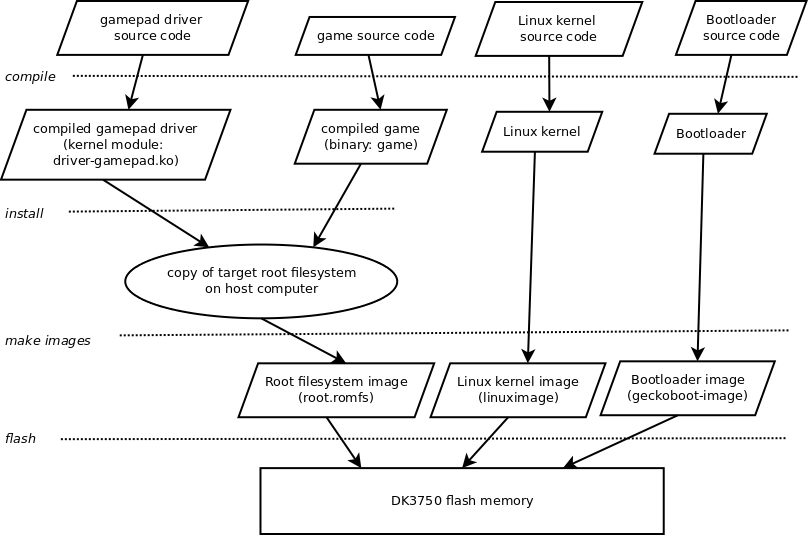
\includegraphics[width=\textwidth]{images/ptxdist_build_process.png}
  \caption{An example overview of a PTXdist build process for a computer game.}
\end{figure}

